\chapter{Formatting Text}
\label{formatting}

\section{Emphasis}

Sometimes you need some extra punch to get your point across.
The simplest way to emphasize text in \LaTeX{} is with the \verb|\emph| command,
which \emph{italicizes} its argument:
\begin{leftfigure}
\begin{lstlisting}
\emph{Oh my!}
\end{lstlisting}
\end{leftfigure}
gives us
\begin{leftfigure}
\lm \emph{Oh my!}
\end{leftfigure}
We have more tools at our disposal:
\begin{leftfigure}
\begin{lstlisting}
We can also use \textbf{boldface} or \textsc{small caps}.
\end{lstlisting}
\end{leftfigure}
producing
\begin{leftfigure}
\lm%
We can also use \textbf{boldface} or \textsc{small caps}.
\end{leftfigure}
Be judicious when you use, especially boldface.
It excels at drawing the reader's attention away from everything around it,
so too much is distracting.

\section{Meeting the whole (type) family}

The styles shown above are just a few of the many available to you.
A (mostly) complete list follows:
\begin{flushleftfigure}
\lm%
\begin{tabularx}{0.9\textwidth}{l|l|l}
{\normalfont Command} & {\normalfont Alternative} & {\normalfont Style} \\
\hline
\texttt{\textbackslash textnormal\{...\}} & \texttt{\{\textbackslash normalfont ...\}} & the default \\
\texttt{\textbackslash emph\{...\}} & \texttt{\{\textbackslash em ...\}} & \emph{emphasis, typically italics} \\
\texttt{\textbackslash textrm\{...\}} & \texttt{\{\textbackslash rmfamily ...\}} & roman (serif) type \\
\texttt{\textbackslash textsf\{...\}} & \texttt{\{\textbackslash sffamily ...\}} & {\fontspec{Latin Modern Sans}sans serif type} \\
\texttt{\textbackslash texttt\{...\}} & \texttt{\{\textbackslash ttfamily ...\}} & {\fontspec{Latin Modern Mono}teletype (monospaced)} \\
\texttt{\textbackslash textit\{...\}} & \texttt{\{\textbackslash itshape ...\}} & \textit{italics} \\
% WTF: LuaTeX font loading doesn't seem to know what to do with Latin Modern Roman Slant
\texttt{\textbackslash textsl\{...\}} & \texttt{\{\textbackslash slshape ...\}} & {\fontspec{lmromanslant10-regular}slanted, or oblique type} \\
\texttt{\textbackslash textsc\{...\}} & \texttt{\{\textbackslash scshape ...\}} & \textsc{Small Capitals} \\
\texttt{\textbackslash textbf\{...\}} & \texttt{\{\textbackslash bfseries ...\}} & \textbf{boldface} \\
\end{tabularx}
\end{flushleftfigure}
Prefer the first form (which takes the text to format as an argument)
over the second
(which affect the group they are issued in),
since the former automatically handle any
spacing corrections needed around them.\punckern\footnote{For example,
\textit{italic type} amidst upright type needs to be followed
by a slight amount of additional space, called an ``italic correction''\quotekern.}
However, when formatting multiple paragraphs,
or when defining the style of other commands,\punckern\footnote{%
For instance, this book's section headers are styled with
\texttt{\textbackslash Large\allowbreak\textbackslash itshape}.}
the second variety is the only option.

\section{Sizes}

The font size of \introduce{body text}---that is, your main content---is
usually ten points,\punckern\footnote{The standard digital publishing point,
sometimes called the PostScript point, is \otffrac{1}{72} of an inch.
\LaTeX{}, for historical reasons, defines its point (\texttt{pt})
as \otffrac{100}{7227} of an inch
and the former as ``big points''\quotekern, or \texttt{bp}.
Use whichever you'd like.}
but can be adjusted by passing arguments to
\verb|\documentclass|.\punckern\footnote{Stock \LaTeX{} classes accept
\texttt{10pt}, \texttt{11pt}, or \texttt{12pt} as optional arguments.
KOMA~Script classes accept arbitrary sizes with
\monobox{fontsize=<size>}.}
To scale text relative to this default size, use the following commands:
\begin{flushleftfigure}
\lm%
\renewcommand{\arraystretch}{1.1}%
\begin{tabular}{l l}
\texttt{\textbackslash tiny} & \tiny Example Text \\
\texttt{\textbackslash scriptsize} & \scriptsize Example Text \\
\texttt{\textbackslash footnotesize} & \footnotesize Example Text \\
\texttt{\textbackslash small} & \small Example Text \\
\texttt{\textbackslash normalsize} & \normalsize Example Text \\
\texttt{\textbackslash large} & \large Example Text \\
\end{tabular}
\end{flushleftfigure}
\clearpage
\begin{flushleftfigure}
\lm%
\begin{tabular}{l l}
\texttt{\textbackslash Large} & \Large Example Text \\
\texttt{\textbackslash LARGE} & \LARGE Example Text \\
\texttt{\textbackslash huge} & \huge Example Text \\
\texttt{\textbackslash Huge} & \Huge Example Text \\
\end{tabular}
\end{flushleftfigure}
You'll find some subtleties at play here.
\LaTeX's default type family, Latin Modern,
comes in multiple \introduce{optical sizes}.
Smaller fonts aren't just shrunken versions of their big siblings---they
have thicker strokes, exaggerated features,
and more generous spacing to improve legibility at their size.
\begin{leftfigure}
\fontspec{lmroman5-regular} When I magnify 5 point type
\lm and place the result next to 11 point type,
you can instantly see the differences.
\end{leftfigure}
Optical sizes were standard back when fonts were made out of metal,
but many digital typefaces lack them,
given how much more work it demands from the type
designer.\punckern\footnote{If you are fortunate enough to have
a typeface with multiple optical sizes, \LuaLaTeX{}
and \XeLaTeX{} can make good use of them! See \chapref{fonts}
for more on font selection.}

But points and optical sizes don't tell the whole story.
Each typeface has its own proportions, which make a huge difference
in perceived size.
(Compare Garamond, {\fontspec{Latin Modern Roman} Latin Modern},
and {\fontspec{NHaasGroteskDSPro-45Lt}\addfontfeature{LetterSpace=3}Helvetica}, all at 11 points.)
Shown below are some common terms:
\begin{centerfigure}
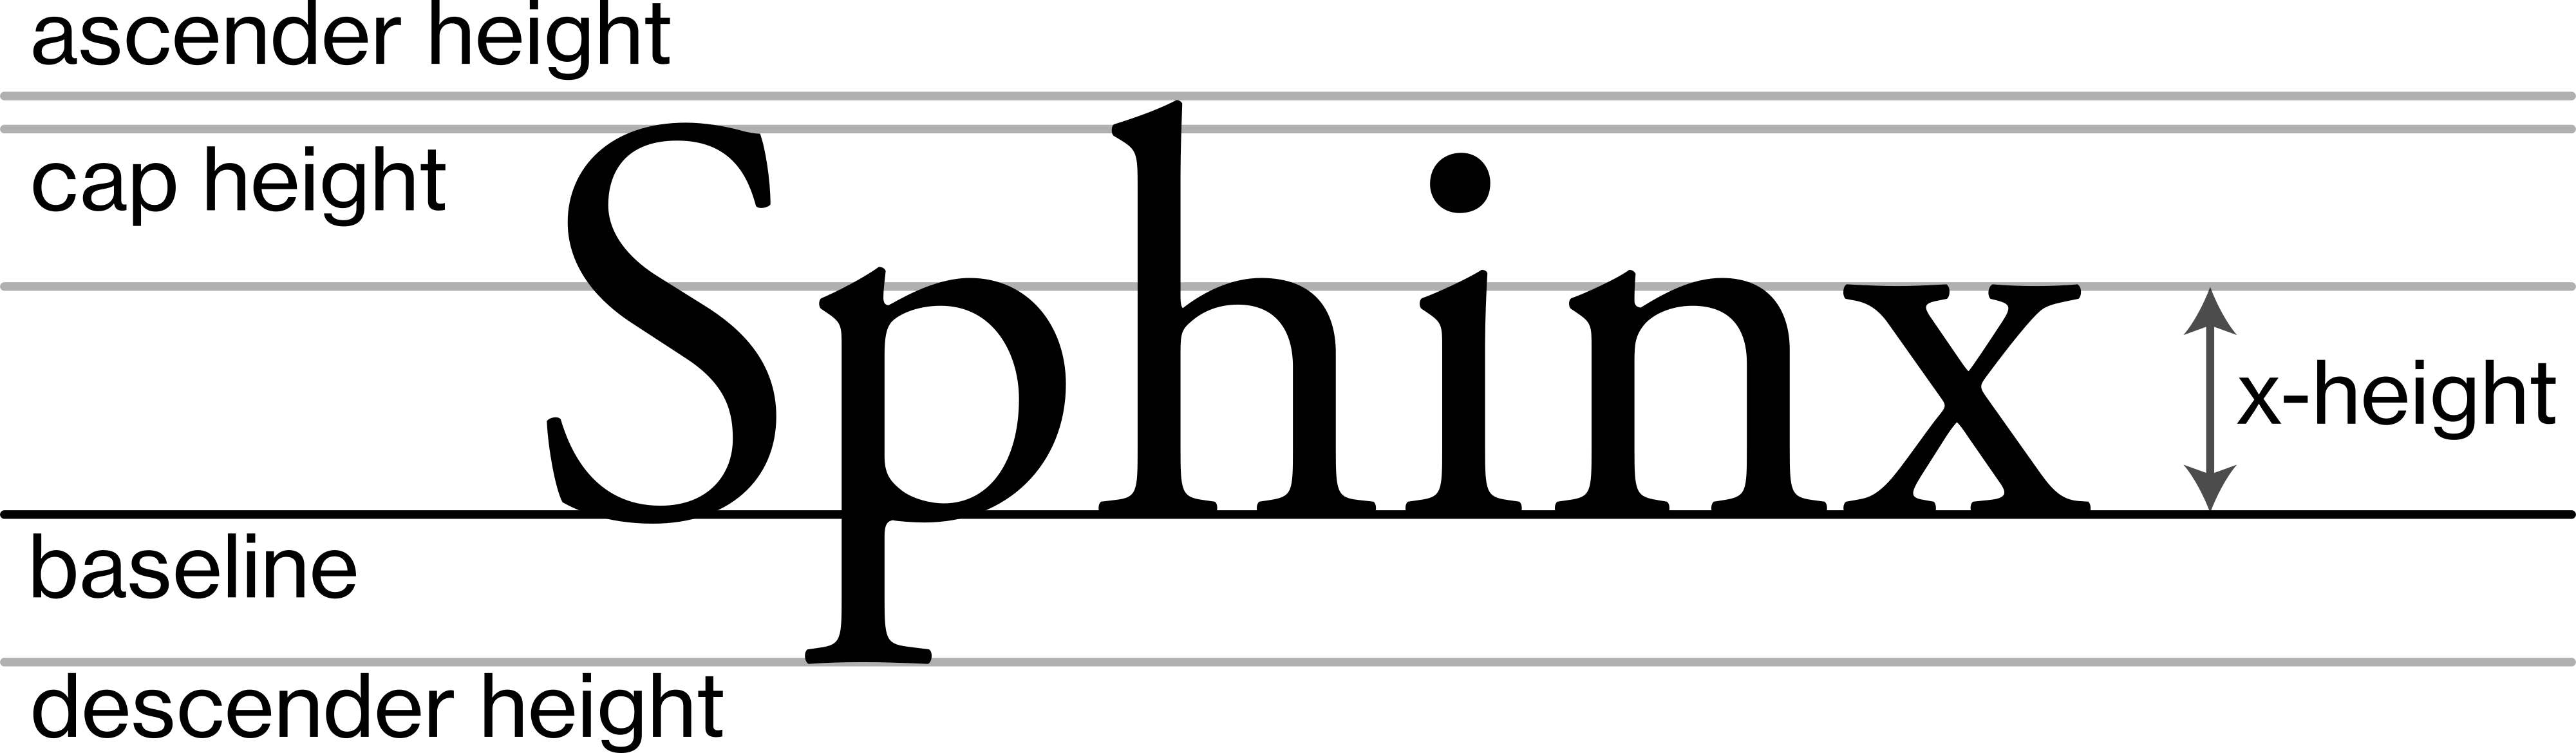
\includegraphics[keepaspectratio,width=0.7\textwidth]{heights.png}

\captionof{figure}{Type sits on the \introduce{baseline},
rises to its \introduce{ascender height},
and drops to its \introduce{descender height}.
The \introduce{cap height} refers to the size of uppercase letters,
and the \introduce{x-height} refers to the size of lowercase letters.}
% For size reference:
%{\sffamily\fontsize{8pt}{8pt}\selectfont This is 8-point text.}
\end{centerfigure}

If the previous commands don't give you a size you need,
you can create custom ones with \verb|\fontsize|,
which takes both a text size and a
distance between baselines.
This must be followed with \verb|\selectfont| to take effect.
For example, \texttt{\textbackslash fontsize\{30pt\}\allowbreak\{30pt\}%
\allowbreak\textbackslash selectfont}
produces
\begin{leftfigure}
\lm
\fontsize{30pt}{30pt}\selectfont
large type with no \\
additional space \\
between lines
\end{leftfigure}
{\fontsize{11pt}{11pt}\selectfont
Note how without a bit of this extra space,
or \introduce{leading},\punckern\footnote{This term comes from the days of
metal type, when strips of lead or brass were inserted
between lines to space them out.\endnote{Jan Middendorp, \textit{Shaping Text}
(Amsterdam, 2014), 71}}
descenders from one line almost collide with ascenders and capitals on
the line below.
Leading is important---without it, blocks of text become uncomfortable to
read, especially at normal body sizes.\par}
Let your type breathe!\footnote{For a discussion of how much leading
to use, see \textit{Practical Typography},
as mentioned in Appendix~\ref{resources}.}

\section{What next?}
\begin{itemize}
\item Learn how to underline text with the \texttt{ulem}
    package.\punckern\footnote{Other typographical tools---like italics,
    boldface, and small caps---are generally preferable to underlining,
    but it has its uses.}
\item Use KOMA~Script to change the size and style of your section headings.
\item Learn the difference between italic and oblique type.
\item Change the default text style
    (used by \verb|\textnormal| and \verb|\normalfont|) by redefining
    \verb|\familydefault|.
\end{itemize}
